\chapter{Appendix}
\section{Class diagram} % Object Model

\begin{figure}[htb]
	\centering
	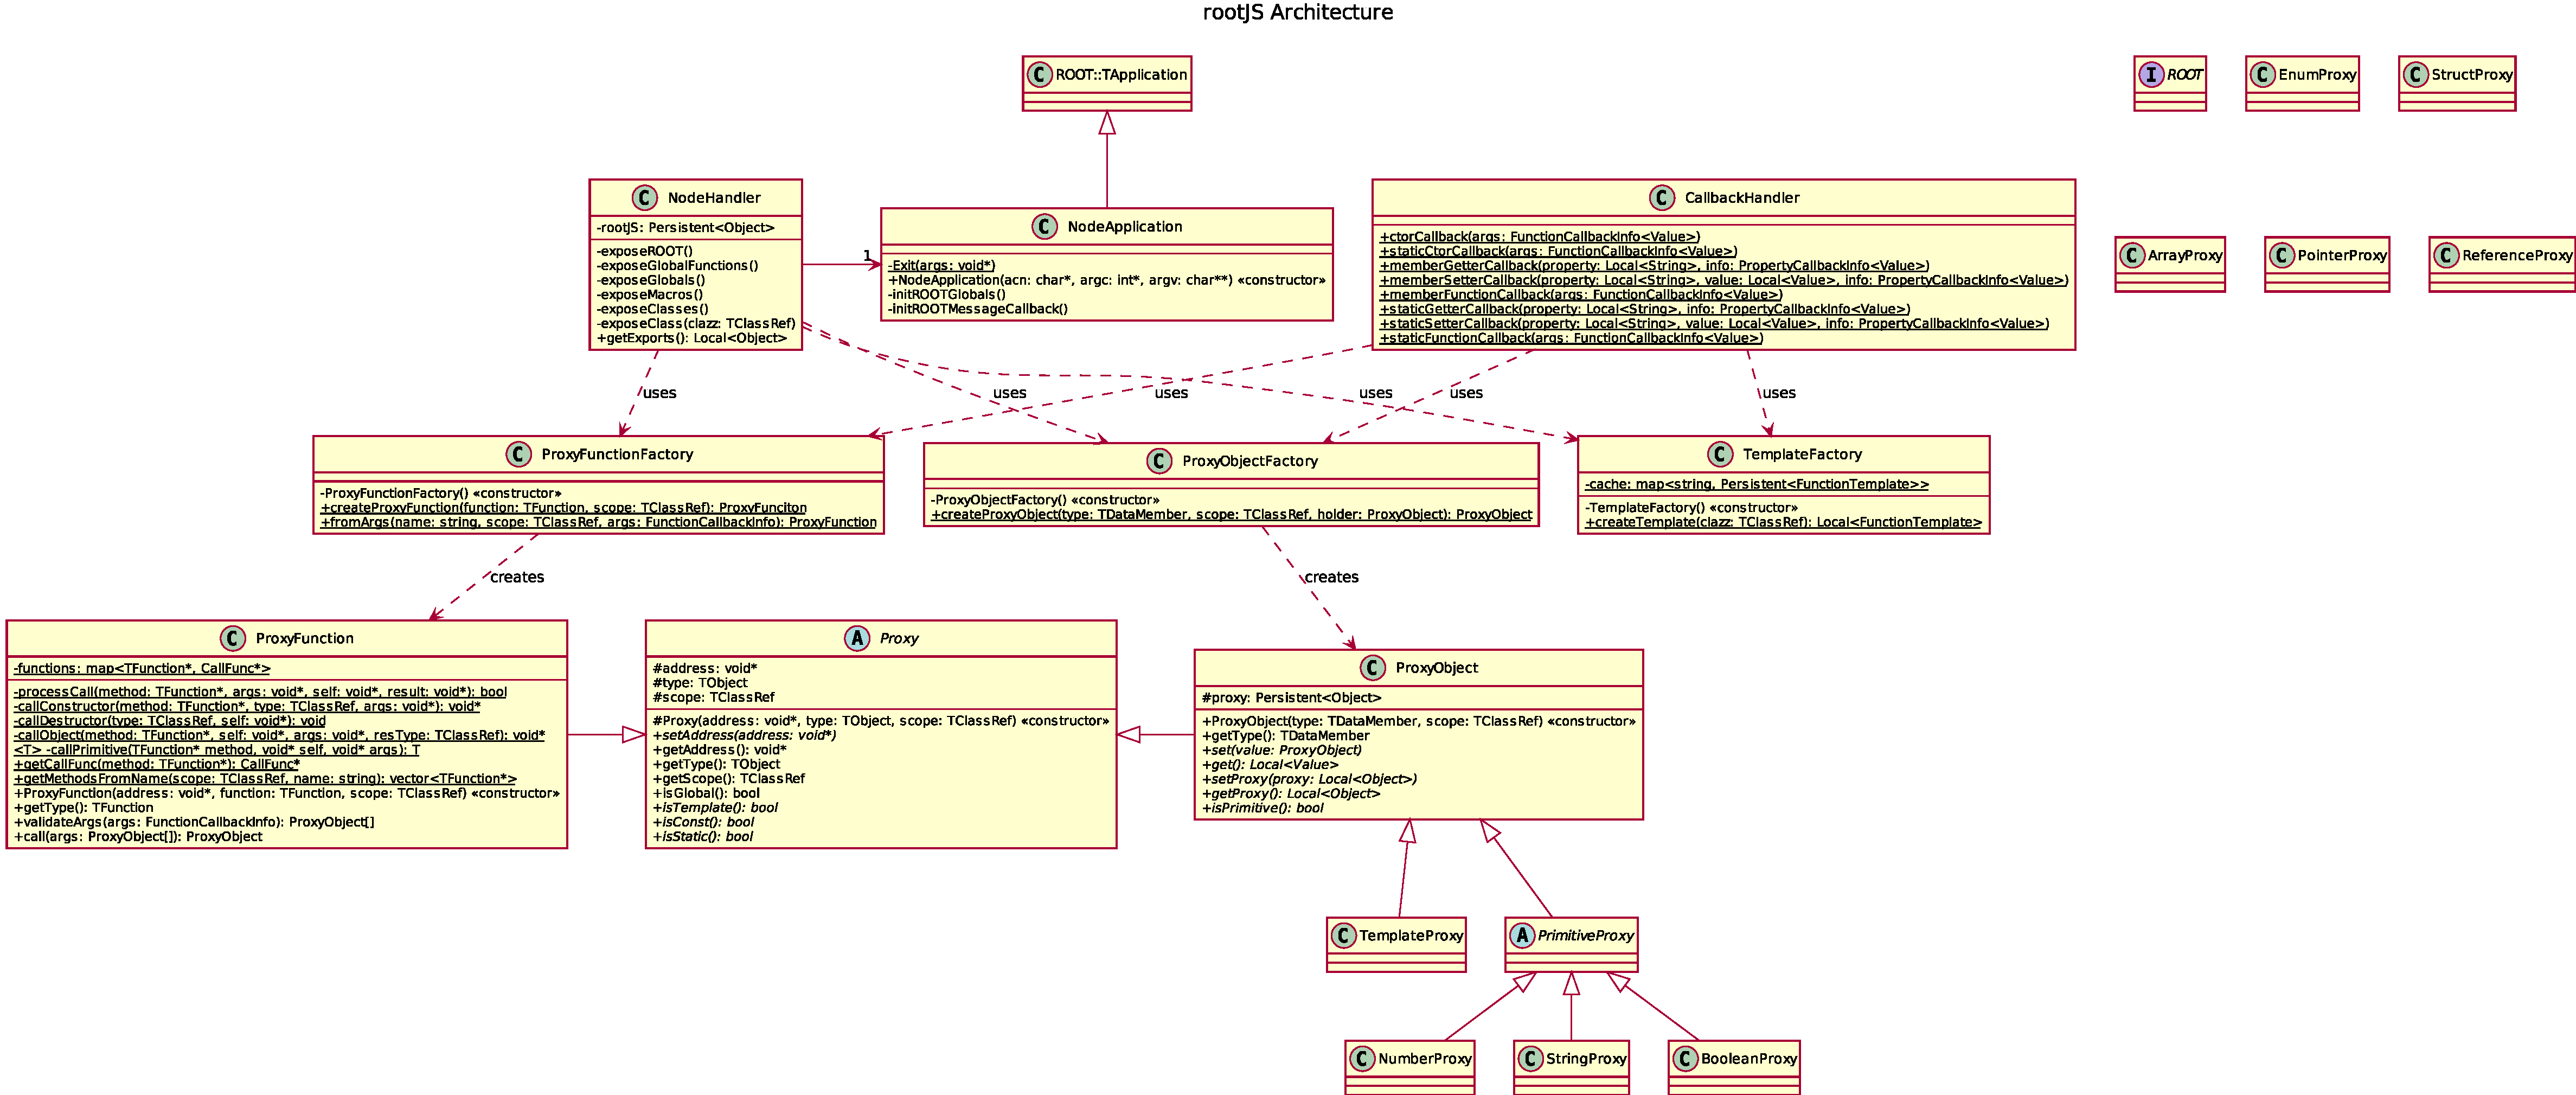
\includegraphics[width=\textheight, height=\linewidth, angle={90}, keepaspectratio]{./latex/resources/architecture.pdf}
	\caption{rootJS class diagram}
\end{figure}

\pagebreak

\section{Dynamic Model}

\begin{figure}[htb]
	\centering
	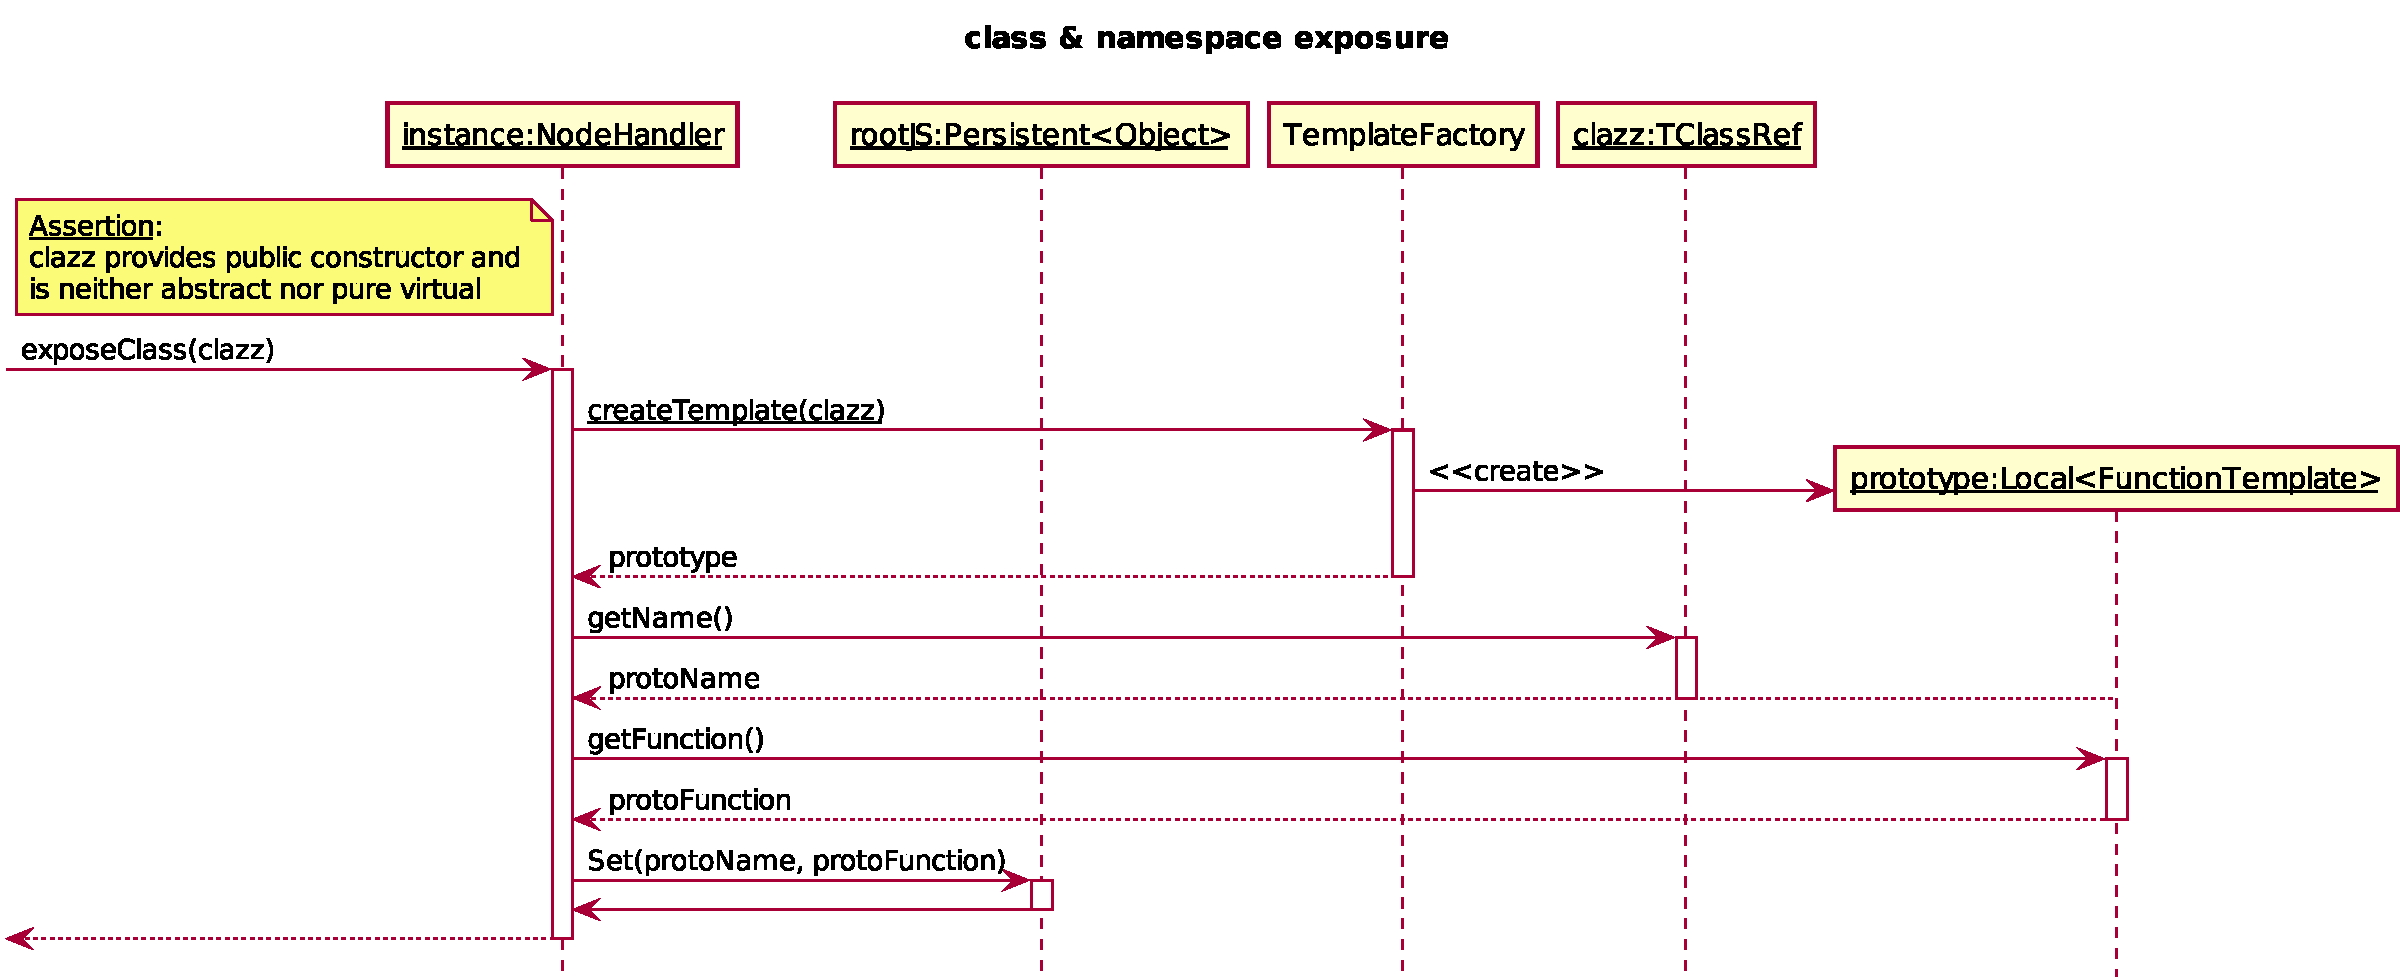
\includegraphics[width=18cm]{./latex/resources/classExposureSequence.pdf}
	\caption{class exposure sequence}
\end{figure}

\begin{figure}[htb]
	\centering
	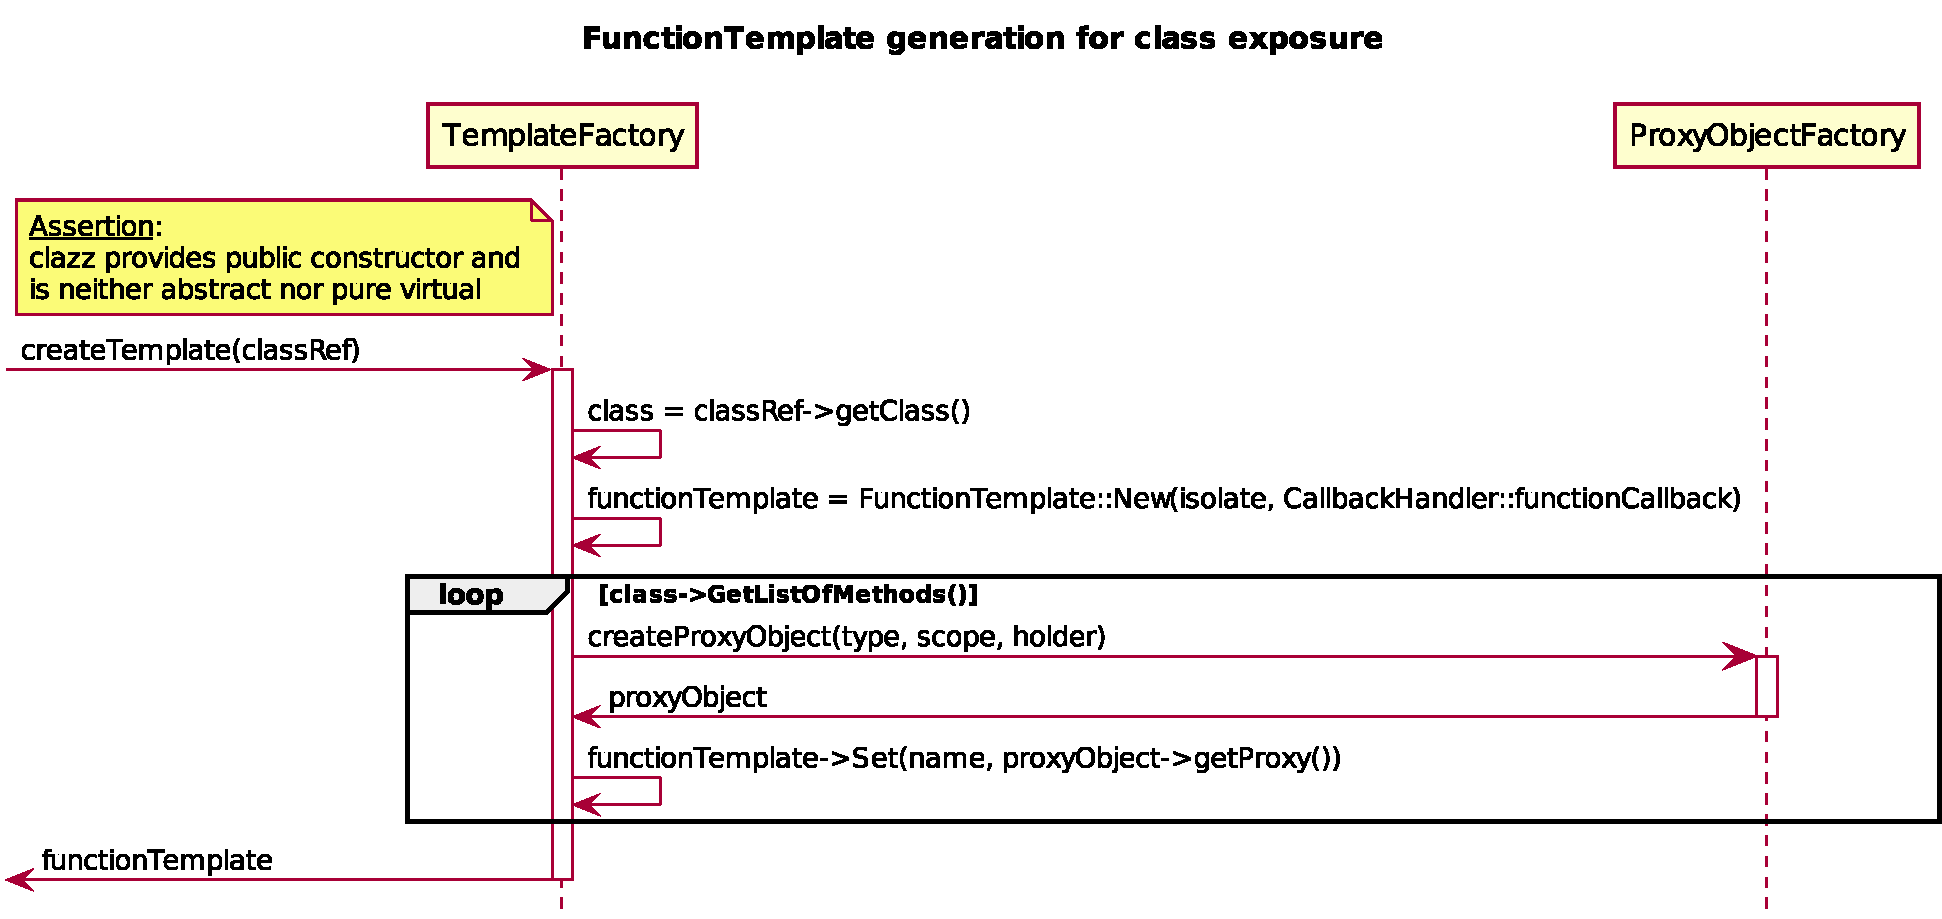
\includegraphics[width=18cm]{./latex/resources/functionTemplateGenerate.pdf}
	\caption{class exposure sequence}
\end{figure}

\begin{figure}[htb]
	\centering
	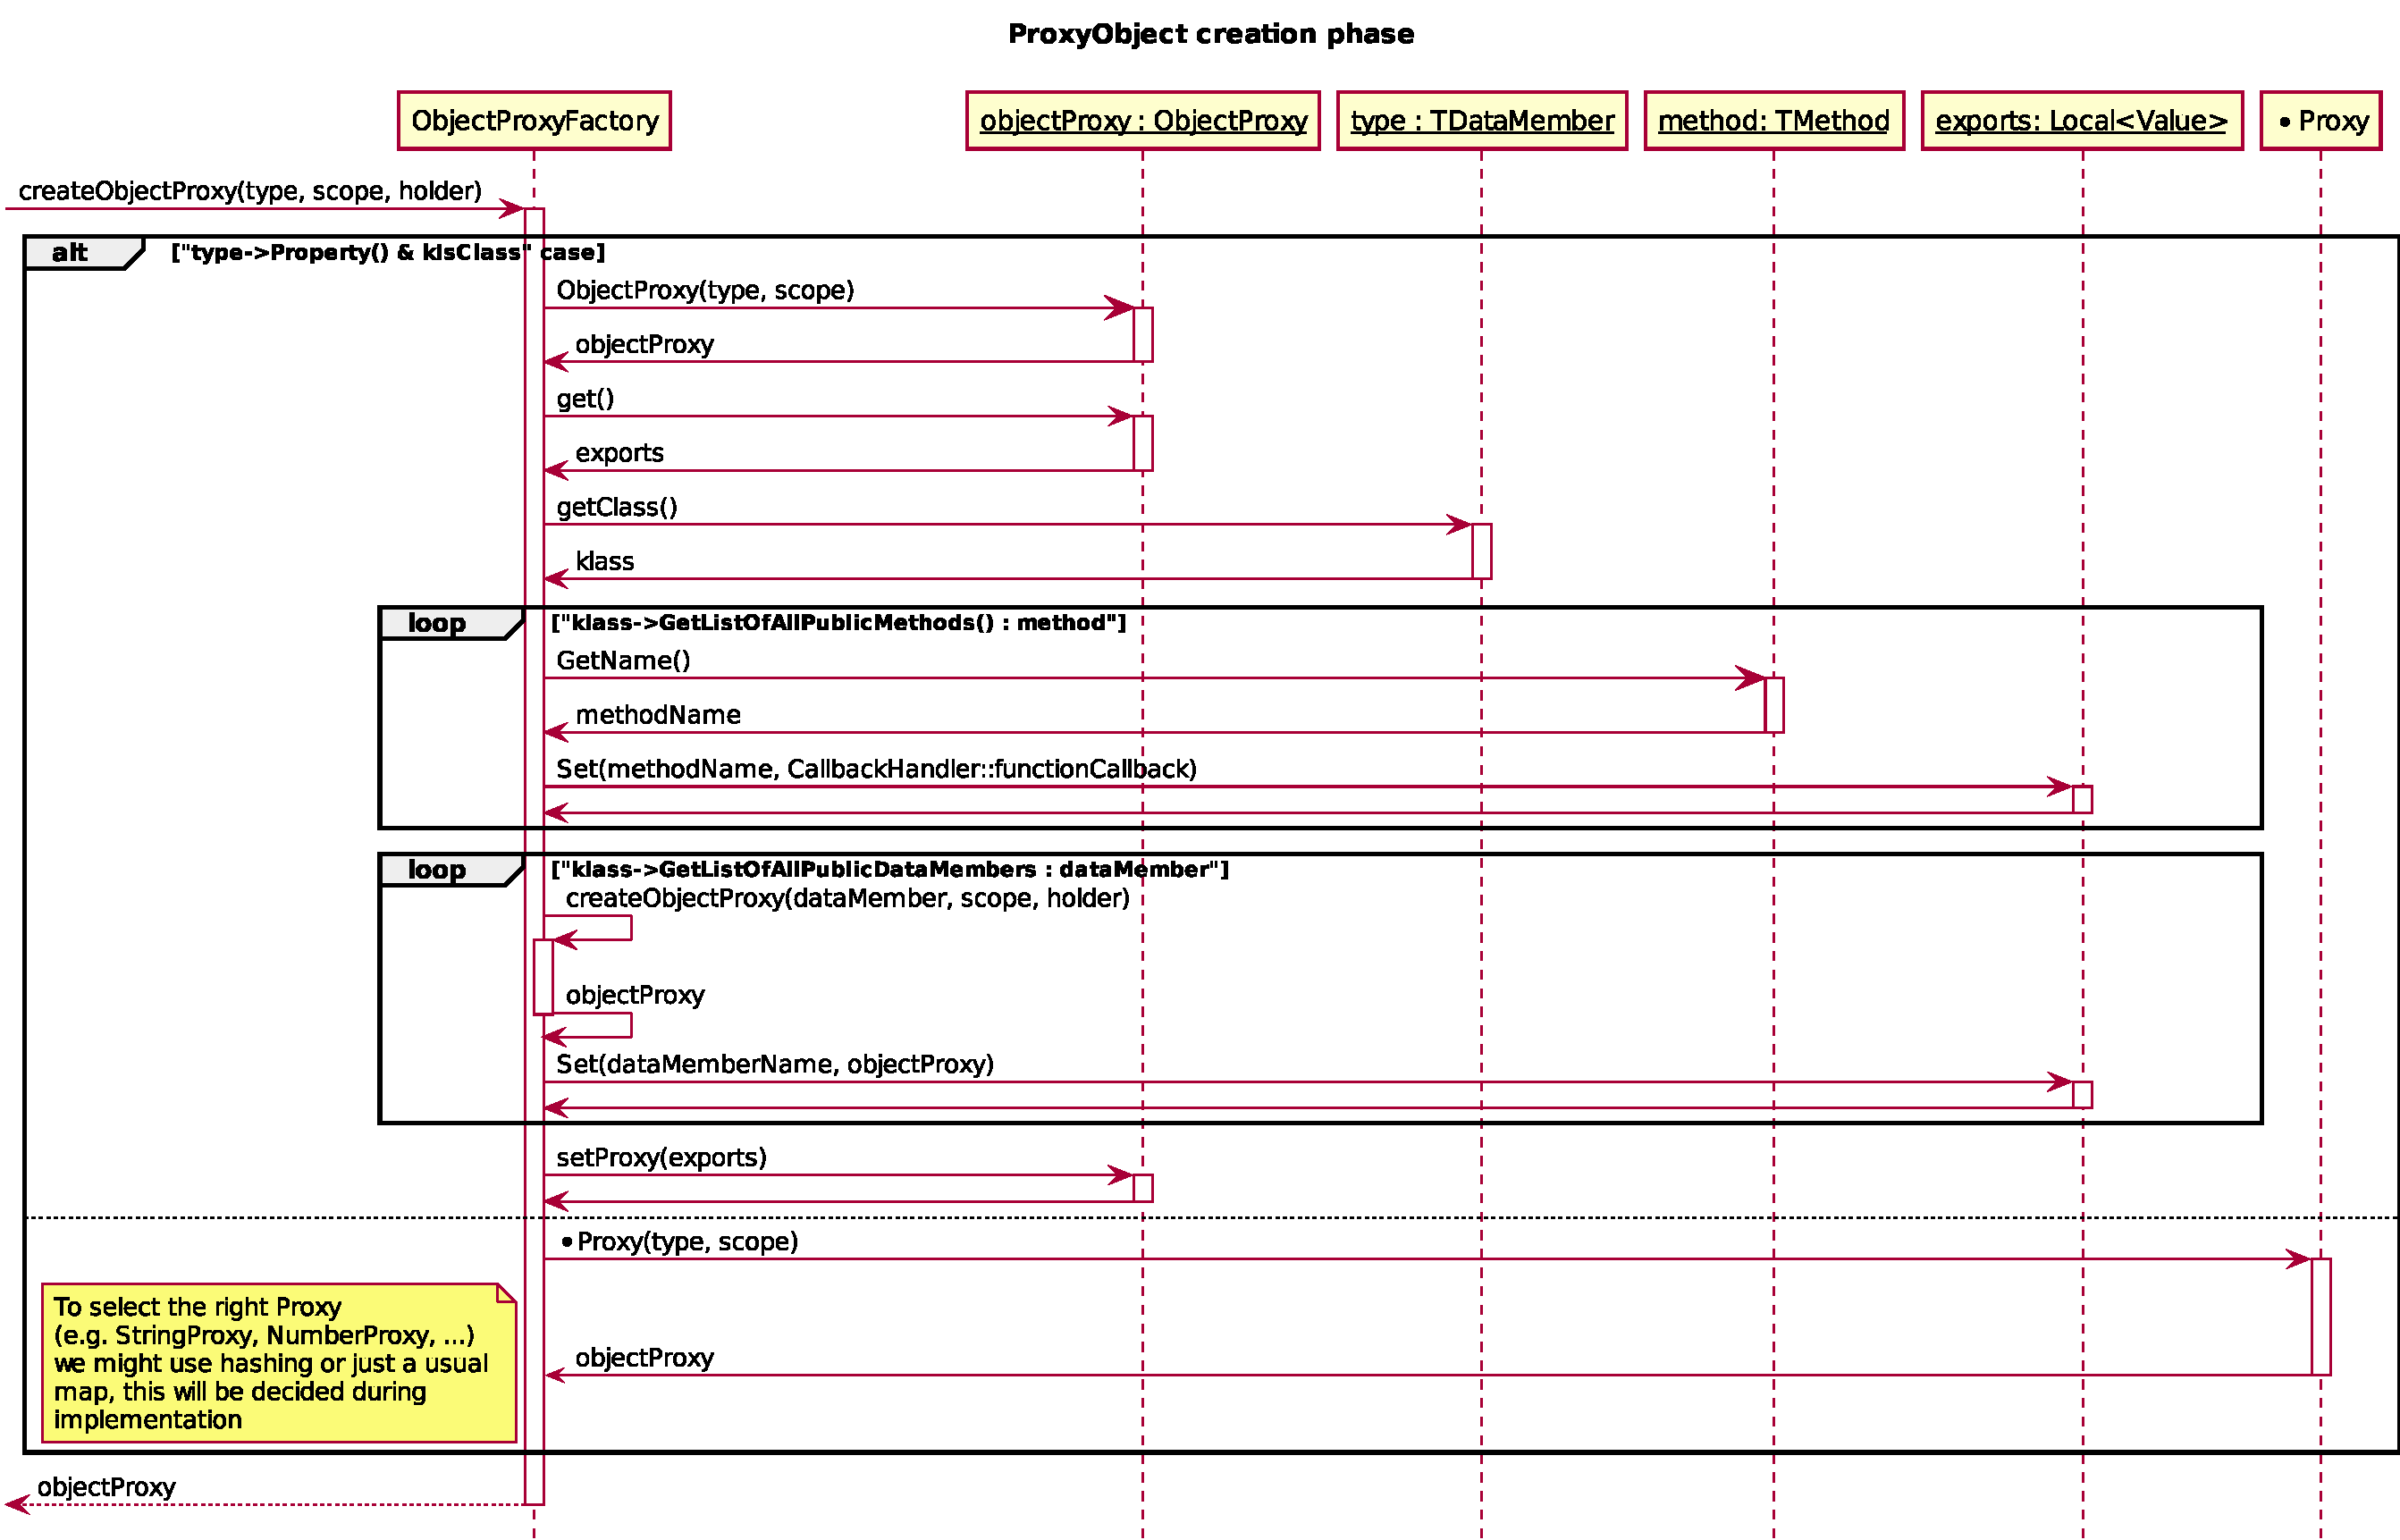
\includegraphics[width=18cm]{./latex/resources/createProxyObject.pdf}
	\caption{ProxyObject creation sequence}
\end{figure}

\newpage

\section{Glossary}
\paragraph{Callback}
A function which is passed as an argument to some code, which is then expected to call the argument back.
\paragraph{Constructor}
A method which is used to create an object.
\paragraph{Encapsulation}
A piece of functionality of certain languages used to restrict access to some of the object's variables and methods
\paragraph{Instance}
A created object.
\paragraph{Proxy}
A class functioning as an intermediary between two classes.
\paragraph{Static}
A method which does not require the object to be instantiated.
\paragraph{Template} 
A feature of C++ that allows classes and functions to operate with generic types.
\paragraph{v8} 
An open source JavaScript engine, written in C++ and made by Google.


